\documentclass{article}

% The area before our main document is called preamble
\title{My first document}
\date{08/05/2020}
\author{Evram Youssef}
%This pakcage removes numbering after equations
\usepackage{amsmath}
%Figures package
\usepackage{graphicx}
%For multiple figures
\usepackage{subcaption}


\begin{document}
% This can be done by adding the \pagenumbering{gobble}
% command and then changing it back to \pagenumbering{arabic} 
% on the next page numbers like so:
    \pagenumbering{gobble}
    \maketitle
    \newpage
    \pagenumbering{arabic}

    \pagenumbering{gobble}
    \tableofcontents
    \listoffigures
    \listoftables
    \newpage
    \pagenumbering{arabic}

% These commands for Sectioning...
% The section commands are numbered and will appear in the table of contents of your document.
% Paragraphs aren't numbered and won't show in the table of contents.
    % \section{}
    % \subsection{}
    % \subsubsection{}

    % \paragraph{}
    % \subparagraph{}
%EXAMPLE
    \section{Section 1}
    Hello World!

    \subsection{Subsection 1.1}
    Structuring a document is easy!

    \subsubsection{Subsubsection}
    More text.

    \paragraph{Paragraph}
    Some more text.

    \subparagraph{Subparagraph}
    Even more text.

    \section{Section 2}
    Hello World 2!

    \subsection{Subsection 2.1}
    Equations:
    %Numbered equation
    
        \begin{equation}
            \frac{n!}{k!(n-k)!} = \binom{n}{k}  
        \end{equation}
        \begin{equation}
            x^\frac{1}{2}  
        \end{equation}
        \begin{equation}
            \frac{\mathrm d}{\mathrm d x} \big( k g(x) \big)
        \end{equation}
    %Unnumbered
        \begin{equation*}
            f(x) = x^2
        \end{equation*}
    
    \section{Math}
    %To write equations withina a sentence
    ...
    This formula $f(x) = x^2$ is an example.
    ...
    \begin{align*}
        f(x) &= x^2\\
        g(x) &= \frac{1}{x}\\
        F(x) &= \int^a_b \frac{1}{3}x^3
      \end{align*}
    
    \section{Figures}
    \begin{figure}[t!]
        %I put \linewidth into the brackets, which means the picture will be scaled to fit the width of the document.
        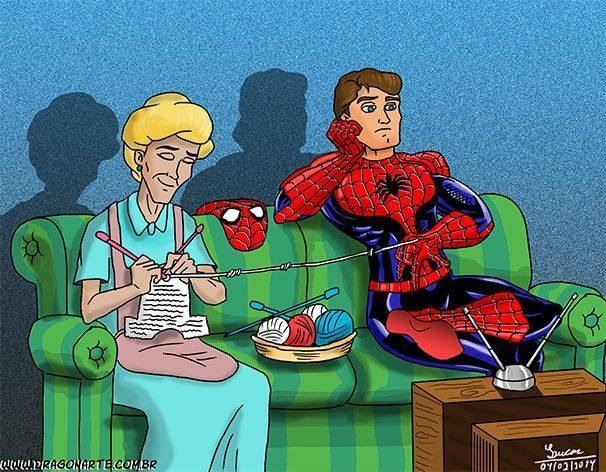
\includegraphics[width=\linewidth]{pic.png}
        \caption{Meme}
        \label{fig:meme}
    \end{figure}

    \begin{figure}[h!]
    \centering
    \begin{subfigure}[b]{0.4\linewidth}
        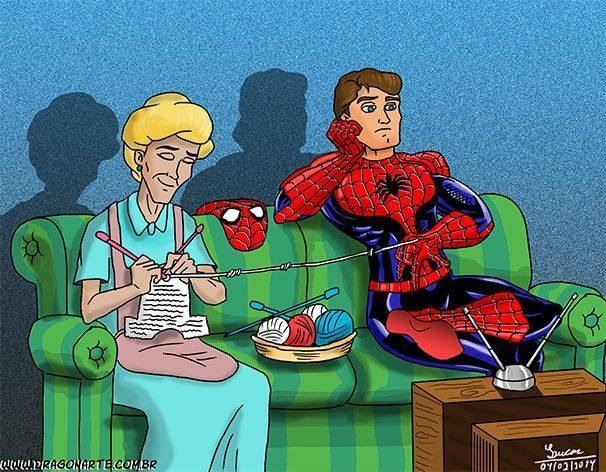
\includegraphics[width=\linewidth]{pic.png}
        \caption{Meme.}
    \end{subfigure}
    \begin{subfigure}[b]{0.4\linewidth}
        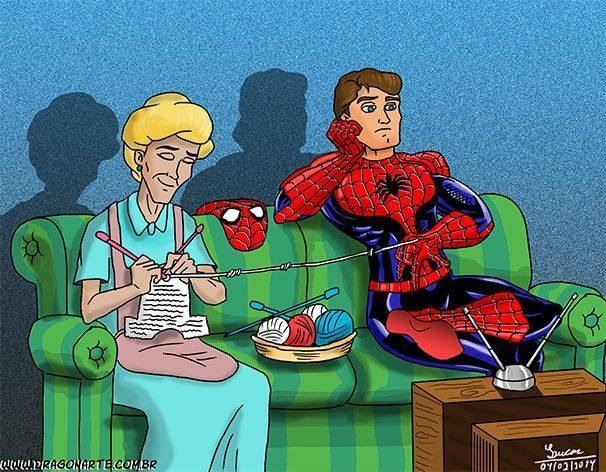
\includegraphics[width=\linewidth]{pic.png}
        \caption{Same Meme.}
    \end{subfigure}
    \caption{The same meme, Two times.}
    \label{fig:coffee}
    \end{figure}




\end{document}